\documentclass[tikz]{standalone}

\begin{document}
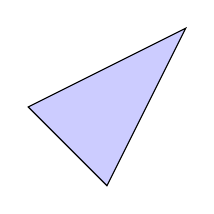
\begin{tikzpicture}

    % \filldraw[red] (0, 0) coordinate(p0) circle (2pt);
    % \filldraw[red] (1,-1) coordinate(p1) circle (2pt);
    % \filldraw[red] (2,1) coordinate(p2) circle (2pt);
    
    % \draw[thick] (p0) -- (p1);
    % \draw[thick] (p1) -- (p2);
    % \draw[thick] (p2) -- (p0);
  
  
    \fill[blue!20] (0, 0) -- (1,-1) -- (2,1) -- cycle;
    \draw[black] (0, 0) -- (1,-1) -- (2,1) -- cycle;
  
    % \filldraw[red] (0, 3) coordinate(p3) circle (2pt);
    % \filldraw[red] (-1, 5) coordinate(p4) circle (2pt);
    % \filldraw[red] (0, 4) coordinate(p5) circle (2pt);
    % \filldraw[red] (1, 4.5) coordinate(p6) circle (2pt);
    
  
    % \draw[thick] (p3) -- (p4);
    % \draw[thick] (p4) -- (p5);
    % \draw[thick] (p5) -- (p6);
    % \draw[thick] (p6) -- (p3);
    
  \end{tikzpicture}
\end{document}